\documentclass[french,10pt]{book}
\input preambule_2014
\input{perso_cecile_2014}

\usepackage{manfnt}

\begin{document}
\renewcommand{\footrulewidth}{0.5pt}

\pieddepage{2014-2015 - 2nde}{Fiche 2 : Inéquations}{\thepage}

\Fiche{2}{Inéquations}

\setlength{\columnseprule}{0pt} % largeur de la ligne entre les deux colonnes

\begin{Exemple*}[s]
    \begin{multicols}{2}
        \begin{enumerate}
            \item Résoudre sur $\R$ $f(x) \geq -1$\par
                \begin{center}
                        \begin{tikzpicture}[scale=0.7,line cap=round,line join=round,>=triangle 45]
                            \draw [color=black,dash pattern=on 2pt off 2pt, xstep=0.7cm,ystep=0.7cm] (-3,-3.5) grid (4,2.5);
                            \draw[->,color=black] (-3,0.0) -- (4,0.0);
                            \foreach \x in {-2,-1,1,2,3}
                            \draw[shift={(\x,0)},color=black] (0pt,2pt) -- (0pt,-2pt) node[below] {\footnotesize $\x$};
                            \draw[->,color=black] (0.0,-3.5) -- (0.0,2.5);
                            \foreach \y in {-3,-2,-1,1,2}
                            \draw[shift={(0,\y)},color=black] (2pt,0pt) -- (-2pt,0pt) node[left] {\footnotesize $\y$};
                            \draw[color=black] (0pt,-10pt) node[right] {\footnotesize $0$};
                            \clip(-3,-3.5) rectangle (4,2.5);
                            \draw[smooth,samples=100,domain=-2.8198332081141952:5.71510293012773] plot(\x,{0.6666666666666666*(\x)^(3.0)-2.0*(\x)^(2.0)-0.6666666666666666*(\x)+1.0});
                            \draw [line width=1.5pt,color=red] (-1.0,0.0)-- (1.0,0.0);
                            \draw [line width=1.5pt,color=red,domain=3.0:5.71510293012773] plot(\x,{0});
                            \draw [line width=1.5pt,color=blue,domain=-2.8198332081141952:5.71510293012773] plot(\x,{-1});
                            \draw (2.5,2) node[anchor=north west] {$\calig{C}_f$};
                            \begin{scriptsize}
                                \draw [line width=1.2pt,color=black] (-1.0,-1.0)-- ++(-1.5pt,-1.5pt) -- ++(3.0pt,3.0pt) ++(-3.0pt,0) -- ++(3.0pt,-3.0pt);
                                \draw [line width=1.2pt,color=black] (1.0,-1.0)-- ++(-1.5pt,-1.5pt) -- ++(3.0pt,3.0pt) ++(-3.0pt,0) -- ++(3.0pt,-3.0pt);
                                \draw [line width=1.2pt,color=black] (3.0,-1.0)-- ++(-1.5pt,-1.5pt) -- ++(3.0pt,3.0pt) ++(-3.0pt,0) -- ++(3.0pt,-3.0pt);
                            \end{scriptsize}
                    \end{tikzpicture}
                \end{center}

On lit les abscisses des points de $\calig{C}_f$ d'ordonnée supérieure ou égale à $-1$\par
L'ensemble des solutions de $f(x) \geq -1$ est $\intervalleff{-1}{1} \cup \intervallefo{3}{+\infty}$.

            \item Résoudre sur $\R$ $f(x) \leq g(x)$. \par
                \begin{center}
                    \begin{tikzpicture}[scale=0.7,line cap=round,line join=round,>=triangle 45]
                        \draw [color=black,dash pattern=on 2pt off 2pt, xstep=0.7cm,ystep=0.7cm] (-3,-3.5) grid (4,2.5);
                        \draw[->,color=black] (-3,0.0) -- (4,0.0);
                        \foreach \x in {-2,-1,1,2,3}
                        \draw[shift={(\x,0)},color=black] (0pt,2pt) -- (0pt,-2pt) node[below] {\footnotesize $\x$};
                        \draw[->,color=black] (0.0,-3.5) -- (0.0,2.5);
                        \foreach \y in {-3,-2,-1,1,2}
                        \draw[shift={(0,\y)},color=black] (2pt,0pt) -- (-2pt,0pt) node[left] {\footnotesize $\y$};
                        \draw[color=black] (0pt,-10pt) node[right] {\footnotesize $0$};
                        \clip(-3,-3.5) rectangle (4,2.5);
                        \draw[smooth,samples=100,domain=-2.8198332081141952:5.71510293012773] plot(\x,{0.6666666666666666*(\x)^(3.0)-2.0*(\x)^(2.0)-0.6666666666666666*(\x)+1.0});
                        \draw [line width=1.5pt,color=red] (0,0.0)-- (3,0.0);
                        \draw [line width=1.5pt,color=red,domain=-3:-1] plot(\x,{(0});
                        \draw [smooth,samples=100,color=blue,domain=-2.8198332081141952:5.71510293012773] plot(\x,{-0.67*(\x)^(2)+1.33*(\x)+1});
                        \draw (2.5,2) node[anchor=north west] {$\calig{C}_f$};
                        \draw [color=blue] (2.7,-2.5) node[anchor=north west] {$\calig{C}_g$};
                            \begin{scriptsize}
                                \draw [line width=1.2pt,color=black] (-1.0,-1.0)-- ++(-1.5pt,-1.5pt) -- ++(3.0pt,3.0pt) ++(-3.0pt,0) -- ++(3.0pt,-3.0pt);
                                \draw [line width=1.2pt,color=black] (0,1)-- ++(-1.5pt,-1.5pt) -- ++(3.0pt,3.0pt) ++(-3.0pt,0) -- ++(3.0pt,-3.0pt);
                                \draw [line width=1.2pt,color=black] (3.0,-1.0)-- ++(-1.5pt,-1.5pt) -- ++(3.0pt,3.0pt) ++(-3.0pt,0) -- ++(3.0pt,-3.0pt);
                            \end{scriptsize}
                    \end{tikzpicture}
                \end{center}

        On lit les abscisses des points de $\calig{C}_f$ situés en dessous ou sur la courbe $\calig{C}_g$\par
        L'ensemble des solutions de $f(x) \leq g(x)$ est $\intervalleof{-\infty}{-1} \cup \intervalleff{0}{3}$.
        \end{enumerate}
    \end{multicols}
\end{Exemple*}



\begin{Exemple*}
    \begin{tikzpicture}[scale=0.7]
        \tkzTabInit[nocadre,espcl=1.5]{$x$/0.75,\small signe de $x-2$/1.3,\small signe de  $-x-3$/1.3,\small signe du  produit/1.3}{$-\infty$,$-3$,$2$,$+\infty$}
        \tkzTabLine{,-,t,-,z,+}
        \tkzTabLine{,+,z,-,t,-}
        \tkzTabLine{,-,z,+,z,-}
    \end{tikzpicture}
\end{Exemple*}

\begin{tikzpicture}[scale=0.7]
\tkzTabInit[nocadre,espcl=1.5]{$x$/0.75,\small signe de $x-2$/1.3,\small signe de  $-x-3$/1.3,\small signe du  produit/1.3}{$-\infty$,$-3$,$2$,$+\infty$}
\tkzTabLine{,-,t,-,z,+}
\tkzTabLine{,+,z,-,t,-}
\tkzTabLine{,-,z,+,z,-}
\end{tikzpicture}

\psframebox[fillstyle=solid,fillcolor=Yellow!30,linewidth=0.4pt,linecolor=Yellow!30,framearc=0.05]{
    \textit{Exemple :}
}
\par\vspace*{-0.25\baselineskip}
\psframebox[fillstyle=solid,fillcolor=Yellow!30,linewidth=0.4pt,linecolor=Yellow!30,framearc=0.05]{
    \begin{minipage}{\linewidth}
        \begin{tikzpicture}
            \tkzTabInit[nocadre,espcl=1.5]{$x$/0.75,\small signe de $x-2$/1.3,\small signe de  $-x-3$/1.3,\small signe du  produit/1.3}{$-\infty$,$-3$,$2$,$+\infty$}
            \tkzTabLine{,-,t,-,z,+}
            \tkzTabLine{,+,z,-,t,-}
            \tkzTabLine{,-,z,+,z,-}
        \end{tikzpicture}
    \end{minipage}
}



\psframebox[fillstyle=solid,fillcolor=Yellow!30,linewidth=0.4pt,linecolor=Yellow!30,]{

    \begin{minipage}{\linewidth}
    \textit{Exemple :}\par 
        \begin{tikzpicture}
            \tkzTabInit[nocadre,espcl=1.5]{$x$/0.75,\small signe de $x-2$/1.3,\small signe de  $-x-3$/1.3,\small signe du  produit/1.3}{$-\infty$,$-3$,$2$,$+\infty$}
            \tkzTabLine{,-,t,-,z,+}
            \tkzTabLine{,+,z,-,t,-}
            \tkzTabLine{,-,z,+,z,-}
        \end{tikzpicture}
    \end{minipage}
}


\psframebox[fillstyle=solid,fillcolor=Yellow!30,linewidth=0.4pt,linecolor=Yellow!30,framearc=0.05]{

    \begin{minipage}{\linewidth}
    \textit{Exemple :}\par 
Test arrondi en fct de la longueur du texte.Test arrondi en fct de la longueur du texte.Test arrondi en fct de la longueur du texte.Test arrondi en fct de la longueur du texte.Test arrondi en fct de la longueur du texte.Test arrondi en fct de la longueur du texte.Test arrondi en fct de la longueur du texte.Test arrondi en fct de la longueur du texte.Test arrondi en fct de la longueur du texte.Test arrondi en fct de la longueur du texte.
    \end{minipage}
}
\end{document} 